\chapter{Main results}

\section{Fairlet decomposition and fair clustering}

Denote:
\begin{itemize}
	\item $\mathcal{Y} = \{ Y_1, \dots, Y_m \}$ is a fairlet decomposition of $X$
	\item $y_j \in Y_j$ is the {\it center} of $Y_j$. (Its choice is arbitrary)
	\item $\beta : X \rightarrow [m]$ is the mapping from a point to the index of the fairlet to which it is mapped.
\end{itemize}

\noindent Then,
\begin{definition}
For a fairlet decomposition $\mathcal{Y}$, define its costs:

\begin{itemize}
	\item $k \text{-median cost} = \sum_{x \in X} d \left(x, y_{\beta(x)}\right) =: \psi(X, \mathcal{Y})$
	\item $k \text{-center cost} = \max_{x \in X} d \left(x, y_{\beta(x)}\right) =: \phi(X, \mathcal{Y})$
\end{itemize}

\noindent Also, we say that a $(b, r)$-fairlet decomposition is {\it optimal} if it has minimum cost among all possible $(b, r)$-fairlet decompositions.
\end{definition}

We shall now see how to reduce this fair clustering to a colorblind clustering.
Recall that a $(t, k)$-fair clustering of $X$ requires that $t \leq \balance(X)$ 
To achieve this, we consider the {\bf vanilla $k$-clustering of the centers of each fairlet} i.e. $k$-clustering of $\{y_1, \dots, y_m\}$.
Then we obtain a set of centers $\{c_1, \dots, c_k\}$ and an assignment function $\alpha_Y : Y \rightarrow [k]$.

Define 
$$\alpha(x) = \alpha_Y(y_{\beta(x)})$$
as the overall assignment function and denote $\mathcal{C}_\alpha$ as the clustering induced by $\alpha$.
Observe that $\balance{C_\alpha} = t$.
As for the cost, refer to the next lemma, which states that the cost is bounded by the sum of costs of vanilla $k$-clustering and the fairlet decomposition:

\begin{lemma}
Denote $\tilde{Y}$ as a multiset where each $y_i$ appears $|Y_i|$ number of times. Then,

$$\psi(X, \mathcal{C}_\alpha) \leq \psi(X, \mathcal{Y}) + \psi(\tilde{Y}, \mathcal{C}_\alpha)$$

$$\phi(X, \mathcal{C}_\alpha) \leq \phi(X, \mathcal{Y}) + \phi(\tilde{Y}, \mathcal{C}_\alpha)$$

\end{lemma}

This lemma, along with previous reasoning, shows that the fair clustering problem can be reduced to
\begin{itemize}
	\item Find a good fairlet decomposition ($\alpha$-approximation)
	\item Solve the vanilla clustering problem on the centers of the fairlets ($\beta$-approximation)
\end{itemize}
, which is a $(\alpha + \beta)$-approximation in total!



\section{Algorithms}

\subsection{(1, k)-fair center problem}

Let us first consider the case when $\balance(X) = 1$. To find a perfectly balanced clustering, we shall be utilizing a good $(1, 1)$-fairlet decomposition!

Below lemma tells us that finding an optimal $(1, 1)$-fairlet decomposition is not too heavy on computation:

\begin{lemma}
An optimal $(1, 1)$-fairlet decomposition for $k$-center can be found in polynomial time.
\end{lemma}

%\begin{proof}
%This can be proved by relating the above problem to a {\it graph covering problem}.
%Denote $B(X) = \{b_i\}_i$ and $R(X) = \{r_j\}_j$ and create a weighted, {\it complete} bipartite graph $G = (B, R, E)$ with the weight function $w(b_i, r_j) = d(b_i, r_j)$.
%
%Then every $(1, 1)$-fairlet decomposition corresponds to some {\bf perfect matching} in $G$ where each edge represents a fairlet, $Y_i$.
%Letting $\mathcal{Y} = \{Y_i\}_i$, the $k$-center cost $\phi(X, \mathcal{Y})$ is exactly the cost of the maximum weight edge in the matching.
%This can be done in $O(n^2)$ time (cf. "threshold graph", binary searching).
%For each $Y_i$, arbitrarily set one of the two nodes of the corresponding edge as the center, $y_i$, and we are done.
%\end{proof}

Recall that any fair solution induces a set of minimal fairlets. Thus, the cost of the fairlet decomposition found is at most {\it twice} the cost of an optimal solution to the clustering.
	
\begin{lemma}
Let $\mathcal{Y}$ be the partition found previously, and let $\phi_t^*$ be the cost of the optimal $(t, k)$-fair center clustering. Then,
$$\phi(X, \mathcal{Y}) \leq 2 \phi_t^*$$.
\end{lemma}

\begin{remark}
In the paper (Lemma 8), there is no $2$ in the LHS of the inequality.  \cite{Rosner2019} has observed that the fairlet decomposition cost should be bounded by the maximal diameter of a fair clustering, not the radius.
He then gave an example where the above equality holds, thus disproving the original statement:
\begin{figure}[hbt!]
	\centering
	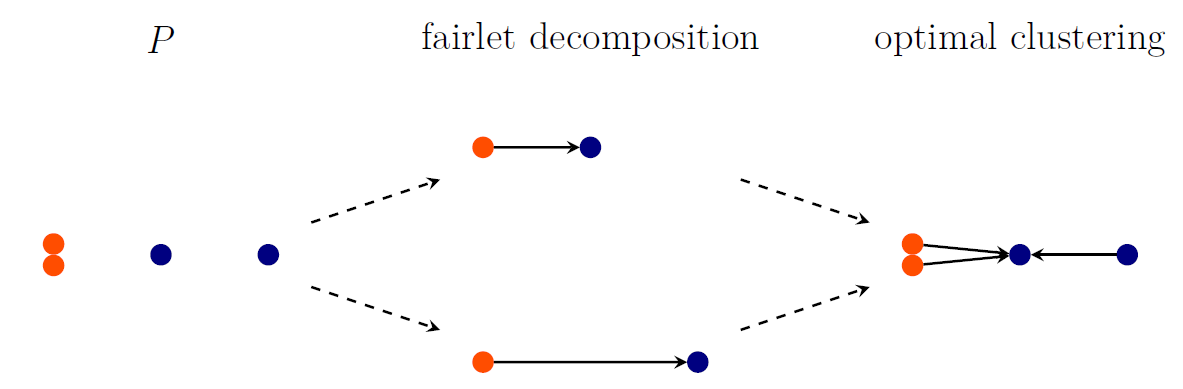
\includegraphics[height=3cm]{results/fig/correction.png}
	\caption{An instance where $\phi(X, \mathcal{Y}) = 2 \phi_t^*$}
\end{figure}
\end{remark}

	
As a final touch, let us utilize a result by Gonzalez for the vanilla $k$-center problem\cite{Gonzalez1985}:

\begin{theorem}[Gonzalez, 1985]
There is an algorithm which, given a $k$-center instance $\mathcal{I}$, produces a $2$-approximation solution to $\mathcal{I}$ in running time $O(kn)$
\end{theorem}

\noindent Combining above discussions, we have the following:

\begin{theorem}
The algorithm that first finds fairlets and then clusters them is a $4$-approximation for the $(1, k)$-fair center problem.
\end{theorem}


\subsection{(1/t', k)-fair center problem}

Now let us consider the case when $\balance(X) = t < 1$. For simplicity, assume that $t = 1/t'$ for some integer $t' > 1$ (as done in the paper)
As a generalization of previous argument, we shall transform this problem into a {\bf minimum cost flow problem (MCFP)}.

\begin{definition}
A {\it flow network} is a directed graph $G = (V, E)$ with a source vertex $s \in V$ and a sink vertex $t \in V$,
where each edge $(u, v) \in E$ has capacity $c(u, v) > 0$, flow $f(u, v) \geq 0$ and cost $a(u, v) \in \mathbb{R}$

\end{definition}

Now let us define what a MCFP is:

\newpage
\begin{problem}[Minimum Cost Flow Problem (MCFP)]
{\bf Input}: A flow network $(G = (V, E), s, t, c, a)$ (without the flow), $d$

{\bf Constraints}:
\begin{itemize}
	\item Capacity constraints: $f(u, v) \leq c(u, v)$
	\item Skew symmetry: $f(u, v) = -f(v, u)$
	\item Flow conservation: $\forall u \not= s, t \ \sum_{w \in V} f(u, w) = 0$
	\item Required flow from $s$ to $t$: $\sum_{w \in V} f(s, w) = \sum_{w \in V} f(w, t) = d$
\end{itemize}

{\bf Output}: Flow $f(u, v)$ such that $\sum_{(u, v) \in E} a(u, v) f(u, v)$ is minimized

\end{problem}


Let us construct an instance of MCFP corresponding to a clustering instance, with a parameter $\tau > 0$ that is to be determined later. 

First, let us construct a directed graph $H_\tau = (V, E)$ such that:

\begin{itemize}	
	\item Vertex set:
$$V = \{\beta, \rho\} \cup B(X) \cup R(X) \cup \left\{ b_i^j | b_i \in B(X) \right\}_{j \in [t']} \cup \left\{ r_i^j | r_i \in R(X) \right\}_{j \in [t']}$$

	\item Edge set:
	\begin{itemize}
		\item $(\beta, \rho)$ with cost 0 and capacity $\min \left( |B(X)|, |R(X)| \right)$
		\item $(\beta, b_i)$ and $(r_i, \rho)$ for each $b_i \in B(X), r_i \in R(X)$, with cost $0$ and capacity $t' - 1$
		\item $(b_i, b_i^j)$ and $(r_i, r_i^j)$ for each $b_i \in B(X), r_i \in R(X), j \in [t']$, with cost $0$ and capacity $1$
		\item $(b_i^k, r_j^l)$ for each $b_i \in B(X), r_i \in R(X), 1 \leq k, l \leq t'$, with cost $1$ if $d(b_i, r_j) \leq \tau$ and $\infty$ otherwise.
	\end{itemize}
	
\end{itemize}

Define the supply and demand at every node as follows::
\begin{itemize}
	\item Every node in $B(X)$ has a supply of $1$
	\item Every node in $R(X)$ has a demand of $1$
	\item $\beta$ has a supply of $|R(X)|$
	\item $\rho$ has a demand of $|B(X)|$
	\item Every other node has zero supply and demand
\end{itemize}

\begin{figure}[hbt]
  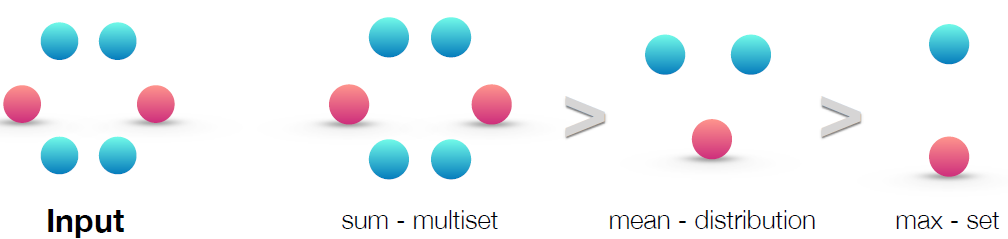
\includegraphics[height=4cm]{results/fig/fig3.png}
\end{figure}


To relate this to our original fair clustering problem, we must be able to build a low cost $(1, t')$-fairlet decomposition, starting from a solution to the described MCF instance.

\begin{lemma}
By reducing the $(1, t')$-fairlet decomposition problem to an MCFP, it is possible to compute a $2$-approximation for the optimal $(1, t')$-fairlet decomposition for the $(1/t', k)$-fair center problem.
\end{lemma}

Combining above with the result by Gonzalez gives:

\begin{theorem}
For any integer $t' \in \mathbb{N}$, the algorithm that first finds fairlets and then clusters them is a $4$-approximation for the $(1/t', k)$-fair center problem.

\end{theorem}


\subsection{(1/t', k)-fair median problem}

Slight modification of previous argument gives us the (approx.) solution for $(t, k)$-fair median problem (with $t = 1/t'$).

For the perfectly balanced case, the modification changes to looking for a {\bf perfect matching of minimum total cost} on the constructed bichromatic graph.
To find $(1, t')$-fairlet decomposition for $t' > 1$, create an instance of MCF, {\it with (some of the) weights as the distances}
	
Let us utilize a result by Li \& Svensson for $k$-median problem\cite{Li2013}:

\begin{theorem}[Li \& Svensson, 2013]
There is an algorithm which, given a $k$-median instance $\mathcal{I}$ and $\varepsilon > 0$, produces a $(1 + \sqrt{3} + \varepsilon)$-approximation solution to $\mathcal{I}$ in running time $O \left( n^{O(1 / \varepsilon^2)} \right)$

\end{theorem}

\noindent Above discussions give the following result:

\begin{theorem}
For any integer $t' \in \mathbb{N}$, the algorithm that first finds fairlets and then clusters them is a $(t' + 1 + \sqrt{3} + \varepsilon)$-approximation for the $(1/t', k)$-fair median problem.

\end{theorem}


\subsection{Hardness}

We now have a theoretical framework and an actual algorithm for solving fair clustering problems. But by taking fairness into account, we have introduced some extra complexity to the classical clustering problems.
As the next theorem shows, ensuring fairness (in clustering) introduces a computational bottleneck! (and a very narrow one, indeed.)

\begin{theorem}
For each fixed $t' \geq 3$,

\begin{itemize}
	\item Finding an optimal $(1, t')$-fairlet decomposition is {\it NP-hard}.
	\item Finding the minimum cost $(1/t', k)$-fair median clustering is {\it NP-hard}
\end{itemize}

\end{theorem}

